%===============================================================
% Template author: Martin Malý.
% Template URL: https://www.overleaf.com/latex/templates/czech-technical-university-colors-beamer-template-lab-of-structure-of-biomolecules/xmgmzfhtyrxt
%===============================================================

\documentclass{beamer}
% \documentclass[aspectratio=169]{beamer} % Uncomment for 16:9
\usepackage[utf8]{inputenc}

\usetheme{Madrid}

\definecolor{cvut_navy}{HTML}{0065BD}
\definecolor{cvut_blue}{HTML}{6AADE4}
\definecolor{cvut_gray}{HTML}{156570}

\setbeamercolor{section in toc}{fg=black,bg=white}
\setbeamercolor{alerted text}{fg=cvut_blue}
\setbeamercolor*{palette primary}{bg=cvut_navy,fg=gray!20!white}
\setbeamercolor*{palette secondary}{bg=cvut_blue,fg=white}
\setbeamercolor*{palette tertiary}{parent=palette primary}
\setbeamercolor*{palette quaternary}{fg=green,bg=gray!5!white}

\setbeamercolor*{sidebar}{fg=cvut_navy,bg=gray!15!white}


\setbeamercolor{titlelike}{parent=palette primary}
\setbeamercolor{frametitle}{parent=palette primary}

\setbeamercolor*{separation line}{}
\setbeamercolor*{fine separation line}{}

\setbeamertemplate{navigation symbols}{}

% Change itemize and enumerate style.
\setbeamertemplate{itemize item}{%
  \textcolor{cvut_navy}{\raisebox{.45ex}{\rule{.8ex}{.8ex}}}
}
\setbeamertemplate{enumerate item}{%
  \textcolor{cvut_navy}{\arabic{enumi}.}
}

\usepackage{eqnarray,amsmath}
\usepackage{amsfonts}
\usepackage{amssymb}
\usepackage{graphicx}
\usepackage{lmodern} % for bold and italic at the same time
\usepackage{bm} % for bold and italic at the same time
\usepackage{epstopdf}
\usepackage{changepage}
\usepackage{array,booktabs}
\usepackage[dua, nolist]{acronym}

%% | -------------------------- tikz -------------------------- |

\usepackage{tikz}
\usepackage{pgfplots}
\pgfplotsset{compat=1.14}
\usetikzlibrary{backgrounds,arrows,automata,shapes,positioning,calc,through,spy,shapes,shapes.geometric,shapes.multipart,fit,patterns,fadings}
\pgfdeclarelayer{background}
\pgfdeclarelayer{foreground}
\pgfsetlayers{background,main,foreground}

% Change color of Figure and Table labels.
\usepackage[labelfont={color=cvut_navy}]{caption}


%====================================================
%========== DEFINITION OF AUTHORS ETC...=============
%====================================================
\author[Yauheni Zviazdou]{Yauheni Zviazdou}
\institute[CTU FEE]{Czech Technical University in Prague \\ Faculty of Electrical Engineering \\ Department of Cybernetics \\}
\title[Text representation models. RAG.]{From FastText to Transformer Models, and their Application in Retrieval-Augmented Generation}
\date[Bachelor's thesis presentation]{Bachelor's thesis presentation\\Supervisor: Ing. Jan Šedivý, CSc.}

%====================================================
%========== BEGINNING OF DOCUMENT ===================
%====================================================
\begin{document}


% Title slide
\begin{frame}
  \titlepage
  \begin{center}
    
\includegraphics[height=2cm]{src/fig/pdfs/ctu_logo_blue_filled.pdf}
  \end{center}
  %!TEX root = ../main.tex

\begin{acronym}
  \acro{CTU}[CTU]{Czech Technical University}
  \acro{API}[API]{Application Programming Interface}
  \acro{RAG}[RAG]{Retrieval-Augmented Generation}
  \acro{NLP}[NLP]{Natural Language Procession}
  \acro{STS}[STS]{Semantic Textual Similarity}
  \acro{QA}[QA]{Question Answering}
  \acro{BERT}[BERT]{Bidirectional Encoder Representations from Transformers}
  \acro{CBOW}[CBOW]{Continuous Bag-of-Words}
  \acro{GloVe}[GloVe]{Global vectors}
  \acro{ML}[ML]{Machine Learning}
  \acro{NN}[NN]{Neural Network}
  \acro{BoW}[BoW]{Bag-of-Words}
  \acro{TF-IDF}[TF-IDF]{Term Frequency-Inverse Document Frequency}
  \acro{OOV}[OOV]{Out of vocabulary}
\end{acronym}

\end{frame}

% Add CTU logo to the all slides excluding title
\logo{
\includegraphics[height=1cm]{src/fig/pdfs/ctu_logo_blue_filled.pdf}}


% Motivation
\begin{frame}
  \frametitle{Motivation}
  \begin{columns}
    \begin{column}{0.5\textwidth}
      \begin{itemize}
        \item LLM chatbots integrate external documents, enhancing context-aware responses.        
        \item Answer quality depends on technical document context.        
        \item Context quality depends on text representation.        
      \end{itemize}
    \end{column}
    \begin{column}{0.5\textwidth}
      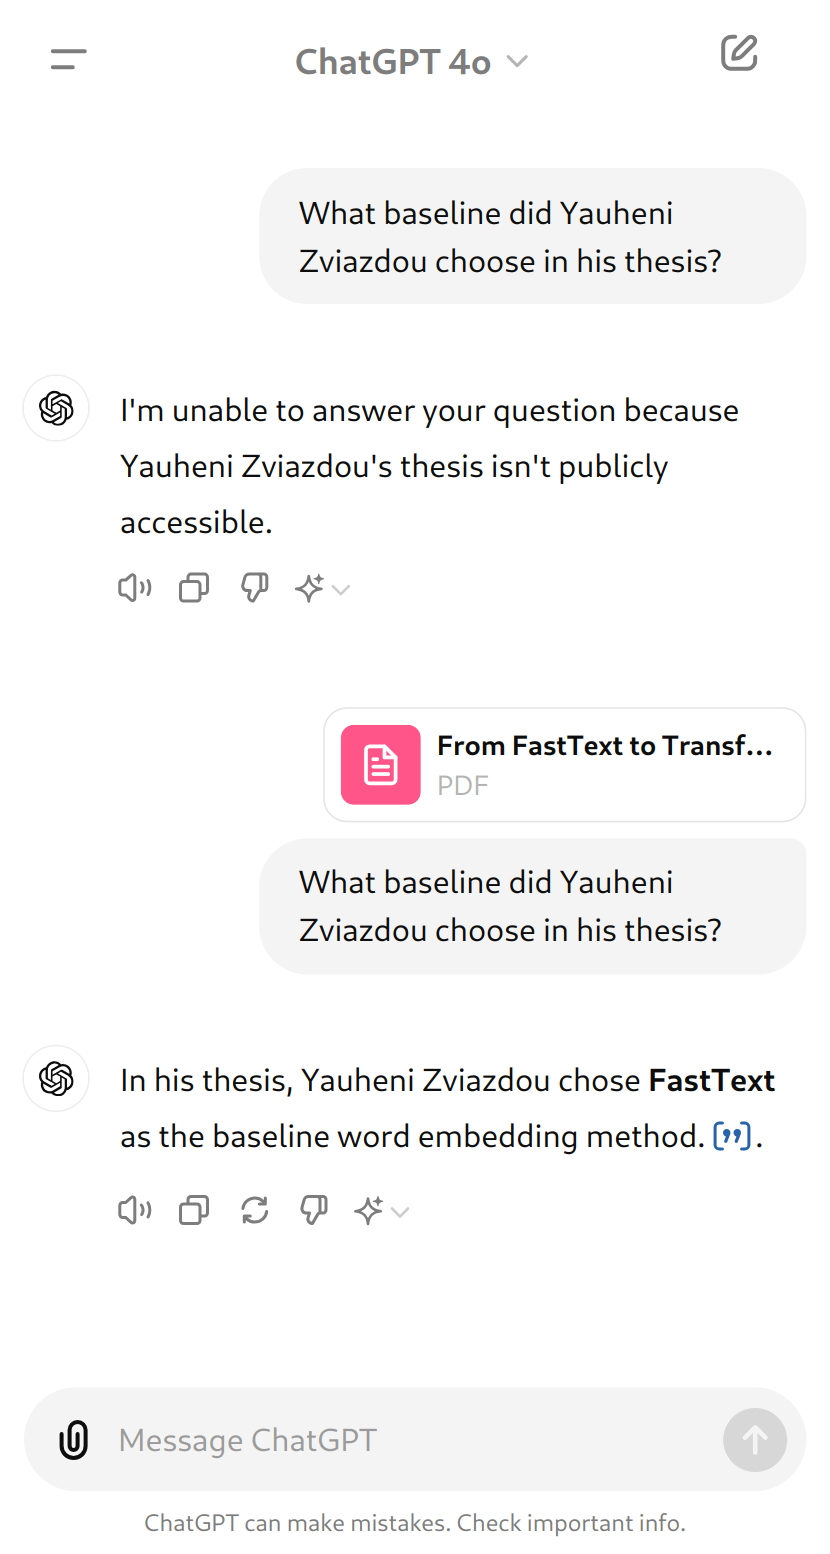
\includegraphics[scale=0.15]{src/fig/imgs/RAG_example.png}
    \end{column}
  \end{columns}
  
  
  
\end{frame}

% Work objectives
\begin{frame}
  \frametitle{Work objectives}
  \textcolor{cvut_navy}{\textbf{Task 1.}} Compare text representation for QA:
  \begin{itemize}
    \item Review text representation methods.
    \item Compare traditional and transformer-based methods.
  \end{itemize}
  \textcolor{cvut_navy}{\textbf{Task 2.}} RAG Optimization
  \begin{itemize}
    \item Choose optimal models for RAG.
    \item Choose optimal chunk size and number of context chunks.
  \end{itemize}
  \bigskip
  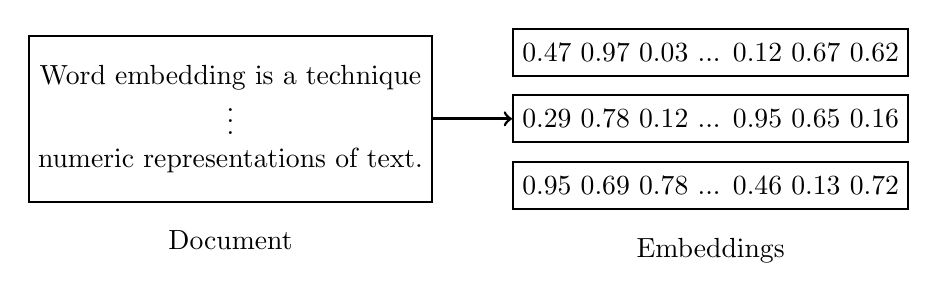
\begin{tikzpicture}[
    longnode/.style={rectangle, draw=black, thick, align=left, minimum height=1.7em, minimum width=14em},
    highnode/.style={longnode, minimum height=6em},
    line width=1pt, black
    ]
    
    %Nodes
    \node[highnode, align=center] (text) []                              {Word embedding is a technique\\ \vdots \\numeric representations of text.};
    \node[longnode, align=center] (emb2) [right=of text]                 {0.29 0.78 0.12 ... 0.95 0.65 0.16};
    \node[longnode, align=center] (emb3) [below=of emb2,yshift=+2.221em] {0.95 0.69 0.78 ... 0.46 0.13 0.72};
    \node[longnode, align=center] (emb1) [above=of emb2,yshift=-2.221em] {0.47 0.97 0.03 ... 0.12 0.67 0.62};

    % Text labels (outside nodes)
    \node[below=of text, yshift=+2.221em]     {Document};
    \node[below=of emb3, yshift=+2.221em]     {Embeddings};

    %Lines
    \draw[->] (text.east) -- (emb2.west);
\end{tikzpicture}

\end{frame}

% Text representation methods
\begin{frame}[t]
  \frametitle{Text representation methods}
  \begin{columns}[onlytextwidth]
    \begin{column}{0.5\textwidth}
      \begin{figure}
        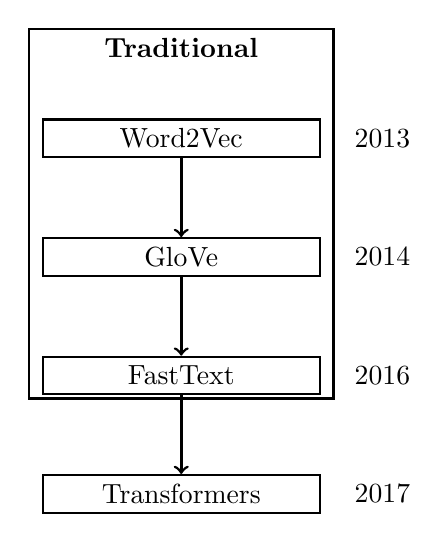
\begin{tikzpicture}[line width=1pt, black]
    %Nodes
    \begin{scope}[every node/.style={rectangle, draw=black, thick, align=left, minimum width=10em}]
    \node (Word2Vec)     []                  {Word2Vec};
    \node (GloVe)        [below=of Word2Vec] {GloVe};
    \node (FastText)     [below=of GloVe]    {FastText};
    \node (Transformers) [below=of FastText] {Transformers};
    \end{scope}

    \node (traditional) [rectangle, draw=black, text depth = 12em, anchor=north, minimum width=11em, yshift=+4em]{\textbf{Traditional}};


    % Text labels (outside nodes)
    \node[right=of Word2Vec.east,xshift=-2.em]     {2013};
    \node[right=of GloVe.east,xshift=-2.em]        {2014};
    \node[right=of FastText.east,xshift=-2.em]     {2016};
    \node[right=of Transformers.east,xshift=-2.em] {2017};

    %Lines
    \draw[->] (Word2Vec.south) -- (GloVe.north);
    \draw[->] (GloVe.south)    -- (FastText.north);
    \draw[->] (FastText.south) -- (Transformers.north);
\end{tikzpicture}
      \end{figure}
    \end{column}
    \begin{column}{0.5\textwidth}
      \textcolor{cvut_navy}{\textbf{FastText}}
      \begin{itemize}
      \item Best traditional method
      \item Uses Machine Learning
      \item Pretrained embeddings, not depends on provided context
      \item Don't capture global information during training (e.g. word order)
      \end{itemize}
      \textcolor{cvut_navy}{\textbf{Transformer models}}
      \begin{itemize}
      \item Use Neural Network with multi-head self-attention mechanism.
      \item Generate embedding depending on provided context.
      \end{itemize}
    \end{column}
  \end{columns}
\end{frame}

% Retrieval-Augmented Generation (RAG)
\begin{frame}
  \frametitle{Retrieval-Augmented Generation (RAG)}
  \begin{columns}[onlytextwidth,T]
    \begin{column}{0.75\textwidth}
      \begin{figure}[h]
        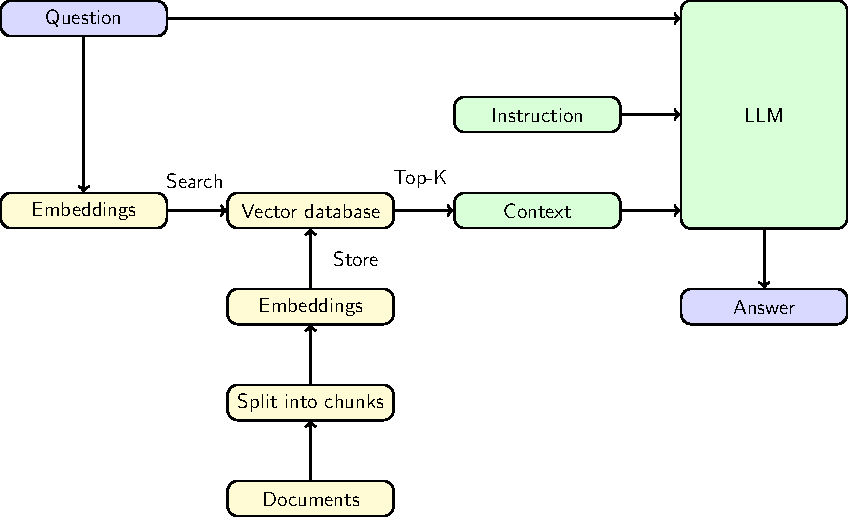
\includegraphics[scale=0.6]{src/fig/pdfs/tikz/RAG_scheme.pdf}
        \caption{Architecture of the RAG algorithm.}
       \end{figure}
    \end{column}

      \begin{column}{0.75\textwidth}
        \textcolor{cvut_navy}{\textbf{Factors}}
        \begin{enumerate}
          \item Embedding \\model
          \item Chunk size
        \end{enumerate}
    \end{column}
  \end{columns}
  
  
\end{frame}

% Methodology
\begin{frame}
  \frametitle{Methodology}
  \begin{columns}[onlytextwidth,T]
    \begin{column}{0.4\textwidth}
      \textcolor{cvut_navy}{\textbf{Corpus information}}
      \begin{itemize}
        \item Czech language
        \item Diacritics, diacriticless
      \end{itemize}
      \textcolor{cvut_navy}{\textbf{Baseline}}
      \begin{itemize}
        \item FastText
        \item Architecture: CBOW
        \item Dimensionality: 300
      \end{itemize}
      \textcolor{cvut_navy}{\textbf{Benchmark}}
      \begin{itemize}
        \item UPV
      \end{itemize}
      \textcolor{cvut_navy}{\textbf{Chosen models}}
      \begin{itemize}
        \item 15 groups
        \item 37 models
        \item 13M - 560M parameters
      \end{itemize}
    \end{column}
    \begin{column}{0.75\textwidth}
      \textcolor{cvut_navy}{\textbf{RAG Components}}
      \begin{itemize}
        \item Embedding model: GTE\textsubscript{Small}
        \item Chunks: 256, 512, 1024, 2048, 4096 char.
        \item Same context size
        \item Answers generation: GPT-3.5-turbo
        \item Answers quality measurement: GPT-4o
      \end{itemize}
      \begin{figure}
        \raggedright
        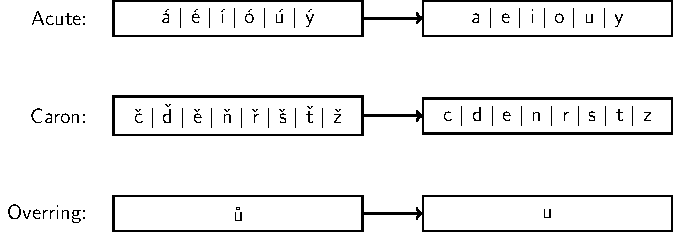
\includegraphics[scale=0.6]{src/fig/pdfs/tikz/diacritics_diacriticless.pdf}
      \end{figure}     
    \end{column}
  \end{columns}
    
  
\end{frame}

% Balanced models
\begin{frame}
  \frametitle{Results: Balanced models}
  \textcolor{cvut_navy}{\textbf{Results analysis}}
  \begin{itemize}
    \item Models with supervised training has best performances.
    \item English-only models has good performances, even without training on Czech.
    \item Task-specified fine-tuning enhance performances.
  \end{itemize}
  \begin{table}
    \centering
    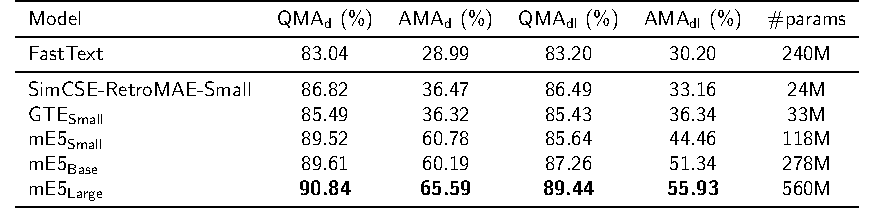
\includegraphics[scale=0.8]{src/fig/pdfs/tables/balanced.pdf}
    \caption{\textcolor{cvut_navy}{\textbf{Balanced models.}}
    Where QMA\textsubscript{d} (QMA\textsubscript{dl}) are Question Matching Accuracy for the diacritics (diacriticless) model.
    AMA\textsubscript{d} (AMA\textsubscript{d}) are Answer Matching Accuracy for the diacritics (diacriticless) model.
    \#params is total number of parameters.}
  \end{table}
\end{frame}

% Optimizing RAG
\begin{frame}
  \frametitle{Results: RAG optimization}
  \begin{table*}[ht!]
    \centering
    \begin{tabular}{lc|ccc}
      \toprule
      $S_{chunk}$ & $K$ & ACC & $t_{encoding}$ \\
      \midrule
      256  & 12 & N/A & 26m 46s \\
      512  & 6  & N/A & 34m 14s \\
      1024 & 3  & N/A & N/A \\
      2048 & 2  & N/A & N/A \\
      4096 & 1  & N/A & N/A \\
      \bottomrule
    \end{tabular}
    \caption{\textbf{RAG evaluation with different parameters.}}
    \label{tab:RAG_evaluation}
  \end{table*}
  
\end{frame}

% Summary
\begin{frame}
  \frametitle{Summary}
  \begin{itemize}
    \item Best models: SimCSE-RetroMAE-Small, GTE\textsubscript{Small}, all mE5 verions.
    \item Best model overall: mE5\textsubscript{Large}.
    \item Best chunk size: 4096 symbols.
  \end{itemize}
  \textcolor{cvut_navy}{\textbf{Thank you for your attention!}}
\end{frame}

\end{document}
% =============================================================
% =========================== END =============================
% =============================================================

